% Appendix Chapter
\chapter*{\textgreek{Παράρτημα Α}}

\pagestyle{fancy}
\fancyhf{}
%\fancyhead[OC]{\leftmark}
\fancyhead[C]{}
%\fancyhead[EC]{\rightmark}
\renewcommand{\footrulewidth}{1pt}
\cfoot{\thepage}

\textgreek{Οι αλγόριθμοι και τα μοντέλα που χρησιμοποιήθηκαν σε αυτή την διπλωματική βρίσκονται στο προφίλ του συγγραφέα στο }Github \textgreek{στον παρακάτω σύνδεσμο} \href{https://github.com/dimimal/semantics_segmentation_of_urban_environments}{link}. \textgreek{Σε αυτό το τμήμα θα δείξουμε το λογισμικό το οποίο υλοποιήθηκε στα πλαίσια της εργασίας για την οπτικοποίηση των αποτελεσμάτων. Το λογισμικό υλοποιήθηκε με την χρήση των βιβλιοθηκών }pyQt4 \cite{pyqt_doc} \textgreek{και} OpenCV \cite{opencv_lib,opencv_man}, \textgreek{ενώ για την υλοποίηση των μοντέλων χρησιμοποιήθηκαν οι βιβλιοθήκες } Keras \cite{keras_bib}, Tensorflow \cite{tensorflow_bib} \textgreek{και} scikit-learn \cite{sklearn_bib}.
\par

\textgreek{Ο πίνακας }\ref{tb:class_colors} \textgreek{επιδεικνύει τα χρώματα που αντιστοιχούν στην κάθε κλάση τα οποία χρησιμοποιούνται στο λογισμικό για την οπτικοποίηση των κλάσεων. Κάθε εικονοστοιχείο το οποίο ανήκει σε κάποια συγκεκριμένη κλάση αντιστοιχεί και το αντίστοιχο χρώμα. }


\begin{table}[H]

\begin{tabular}{|l|l|l|l|l|}
\hline
 \cellcolor[HTML]{804080}\textgreek{Δρόμος} & \cellcolor[HTML]{F423E8}\textgreek{Πεζοδρόμιο} & \cellcolor[HTML]{464646}\textgreek{Κτίριο} & \cellcolor[HTML]{66669C}\textgreek{Τοίχος}& \cellcolor[HTML]{BE9999}\textgreek{Φράχτης}\\ \hline    

\cellcolor[HTML]{999999}\textgreek{Ιστός} & \cellcolor[HTML]{FAAA1E}\textgreek{Φανάρι Κυκλοφορίας} & \cellcolor[HTML]{DCDC00}\textgreek{Πινακίδα Κυκλοφορίας} & \cellcolor[HTML]{6B8E23}\textgreek{Βλάστηση}& \cellcolor[HTML]{98FB98}\textgreek{Έδαφος}\\ 

\cellcolor[HTML]{4682B4}\textgreek{Ουρανός} & \cellcolor[HTML]{DC143C}\textgreek{Άνθρωπος} & \cellcolor[HTML]{FF0000}\textgreek{Αναβάτης} & \cellcolor[HTML]{00008E}\textcolor{white}{\textgreek{Αυτοκίνητο}} & \cellcolor[HTML]{000046} \textcolor{white}{\textgreek{Φορτηγό}} \\

\cellcolor[HTML]{003C64}\textgreek{Λεωφορείο} & \cellcolor[HTML]{005064}\textgreek{Τρένο} & \cellcolor[HTML]{0000E6}\textcolor{white}{\textgreek{Μοτοσυκλέτα}} & \cellcolor[HTML]{770B20}\textgreek{Ποδήλατο} & \cellcolor[HTML]{000000}\textcolor{white}{\textgreek{Κενό}} \\ \hline

\end{tabular}
\caption[\textgreek{Πίνακας Χρωμάτων των Κλάσεων}]{\textgreek{Χρώματα των διαφορετικών αντικειμένων τα οποία φαίνονται στο παρακάτω λογισμικό. }}\label{tb:class_colors}
\end{table}





\textgreek{Το λογισμικό που θα δούμε παρακάτω βασίστηκε στο λογισμικό που έχει δημιουργηθεί από την ομάδα της βάσης δεδομένων }Cityscapes \cite{Cityscapes}.\textgreek{Όπως βλέπουμε στις εικόνες} \ref{fig:viewer_1}, \ref{fig:viewer_2} \textgreek{κατά την εκτέλεση του  προγράμματος εμφανίζεται παράθυρο επιλογής μίας εικόνας για αναγνώριση και ακολουθεί δεύτερο παράθυρο αντίστοιχα για την επιλογή ενός αρχείου/εικόνας το οποίο περιέχει τις προβλέψεις που έχουν παραχθεί από το μοντέλο μας. }
\begin{figure}[H]
 \centering
 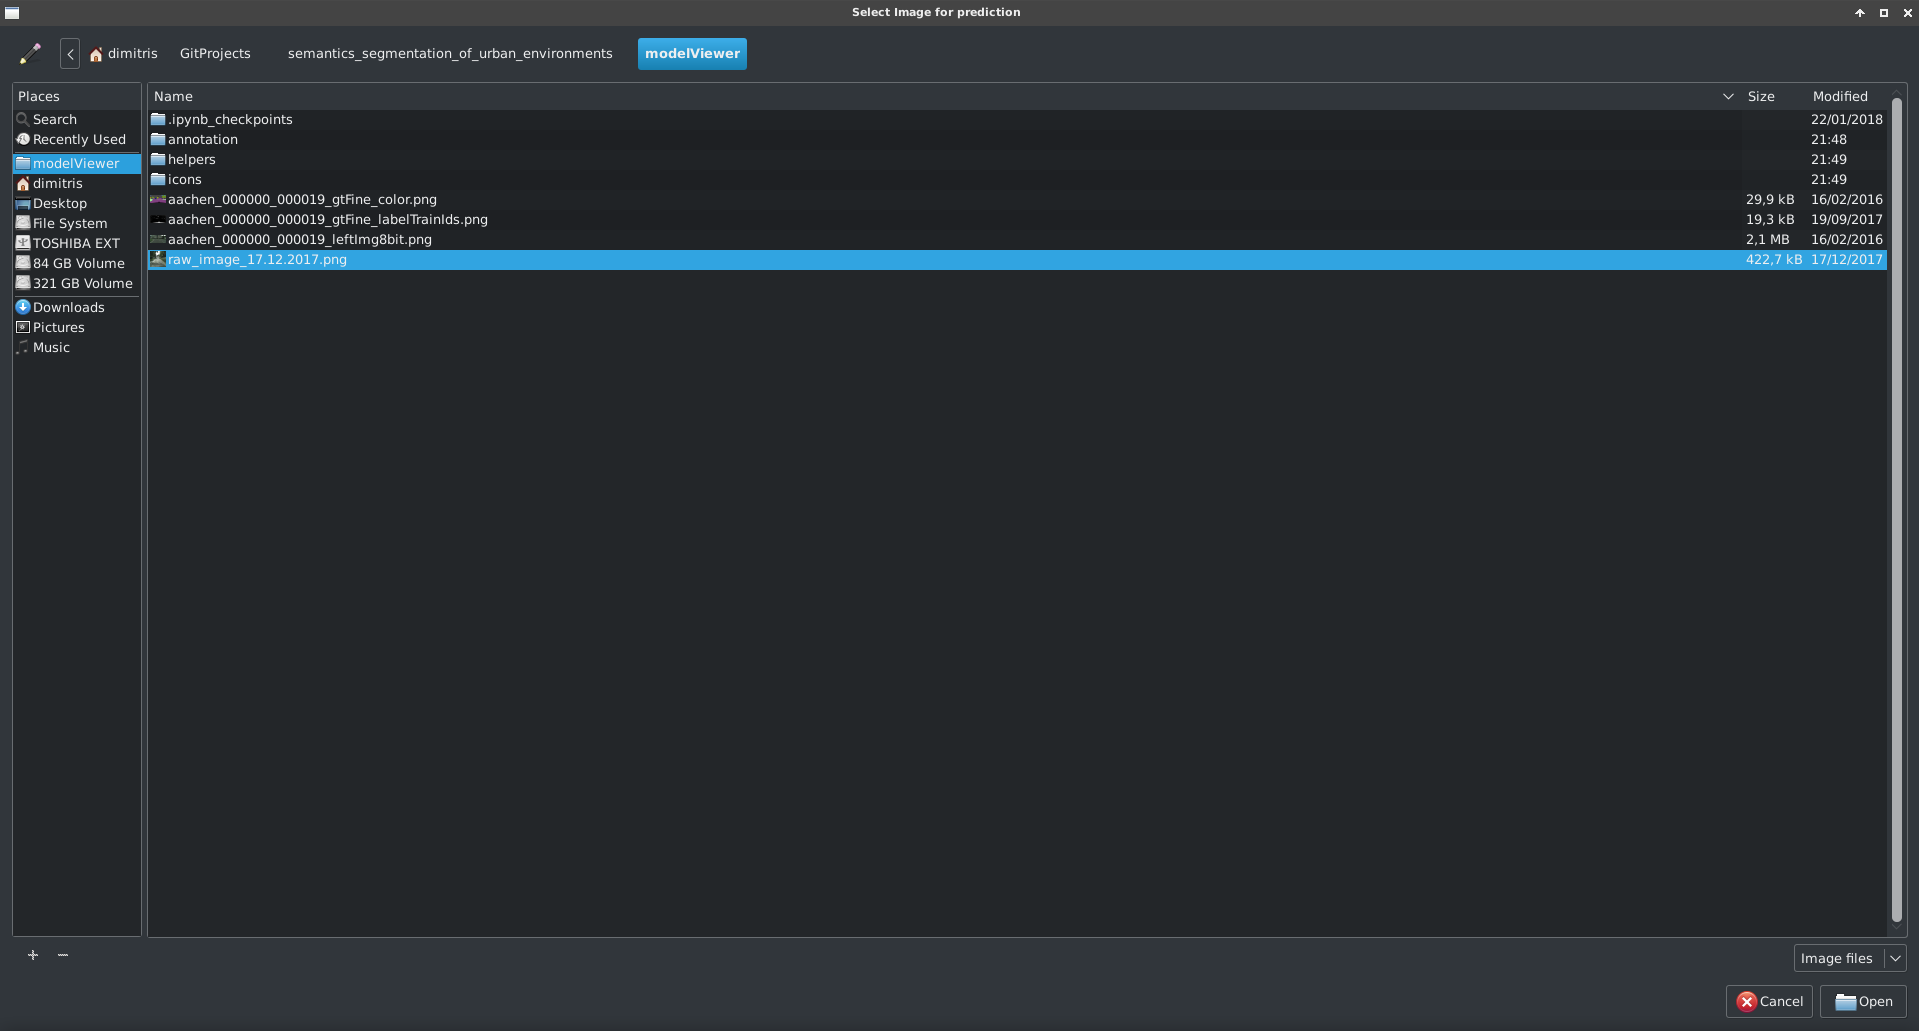
\includegraphics[width=\textwidth, scale=0.3]{Images/viewer_1}
\caption[\textgreek{Επιλογή Εικόνας}]{\textgreek{Επιλογή αρχικής εικόνας για αναγνώριση.}}\label{fig:viewer_1}
\end{figure}

\begin{figure}[H]
 \centering
 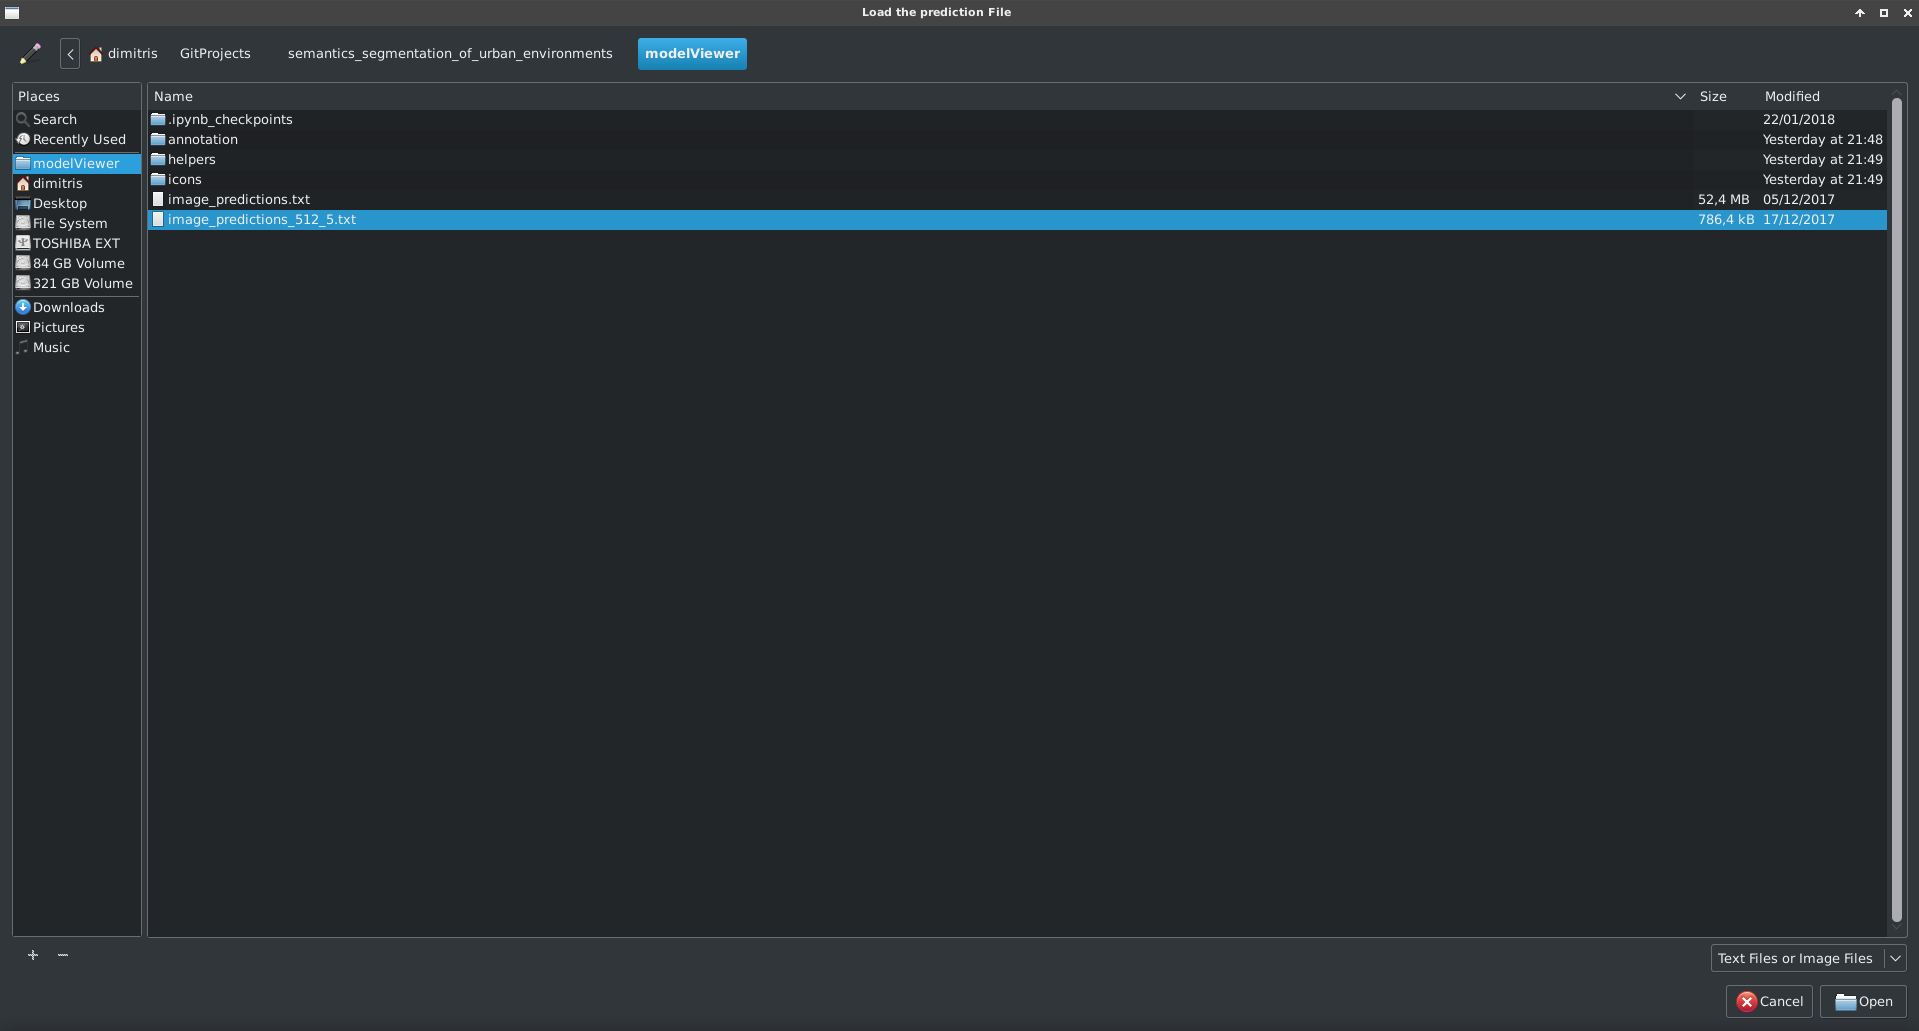
\includegraphics[width=\textwidth, scale=0.3]{Images/viewer_2}
\caption[\textgreek{Επιλογή Αρχείου}]{\textgreek{Επιλογή αρχείου/εικόνας αποτελεσμάτων}}\label{fig:viewer_2}
\end{figure}

\textgreek{Η εικόνα με τις προβλέψεις ζωγραφίζεται πάνω από την εικόνα εισόδου, όπου κάθε κατηγορία αντικειμένων έχει ένα χρώμα που την αντιπροσωπεύει (εικόνες} \ref{fig:viewer_3}\textgreek{ και} \ref{fig:viewer_4}). \textgreek{Ο δείκτης ανάλογα με την θέση του δείχνει με άσπρα έντονα γράμματα στα δεξιά του δείκτη την κατηγορία που ανήκει το εικονοστοιχείο. Επίσης, έχουμε δώσει την εξής λειτουργία, την ρυθμιζόμενη διαφάνεια του στρώματος με τις προβλέψεις για να δώσουμε την ευχέρεια στον χρήστη να επιλέξει την κατάλληλη επιθυμητή διαφάνεια ώστε να μπορεί να διακρίνει ευκολότερα τα αντικείμενα με τις αντίστοιχες κατηγορίες που ανήκουν.}

\begin{figure}[H]
 \centering
 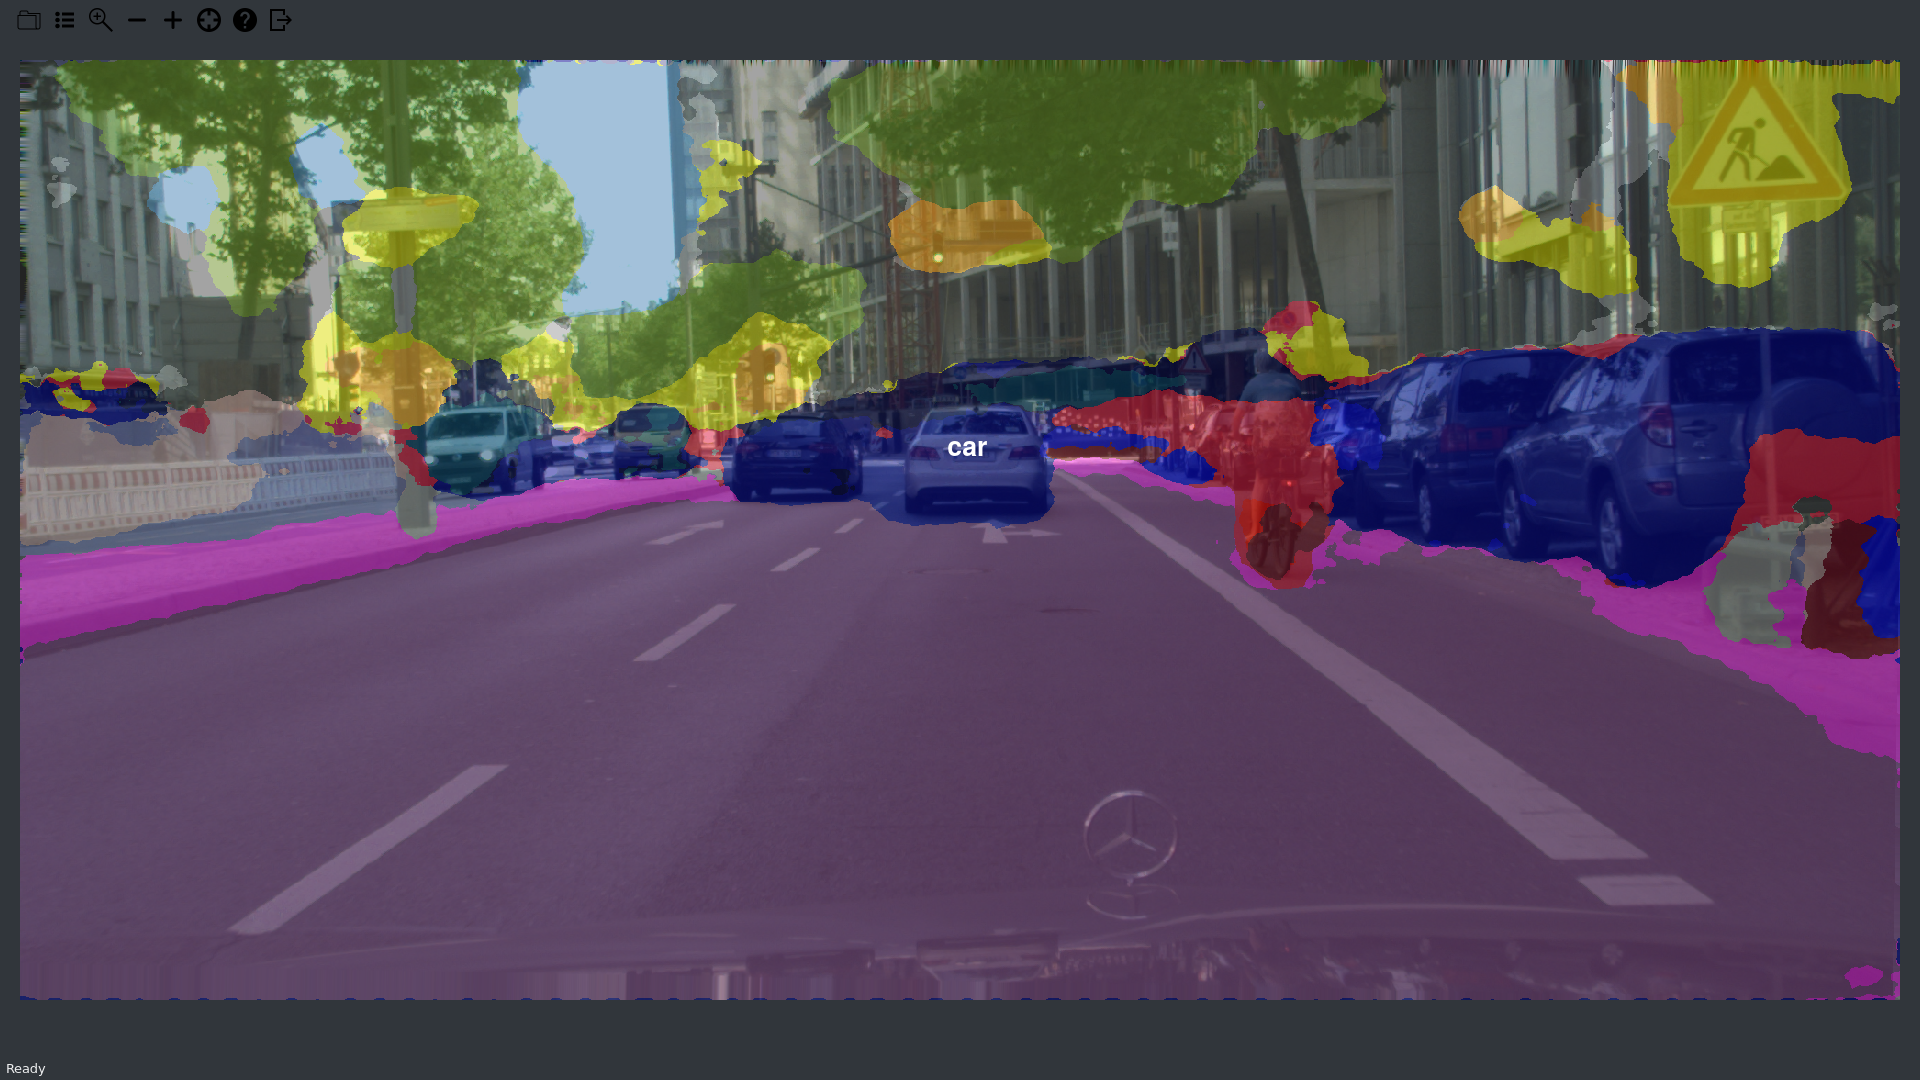
\includegraphics[width=\textwidth, scale=0.3]{Images/viewer_3}
\caption[\textgreek{Προβολή Ετικέτας}]{\textgreek{Προβολή εικόνας και πρόβλεψης του μοντέλου} .}
 \label{fig:viewer_3}
\end{figure}

\begin{figure}[H]
 \centering
 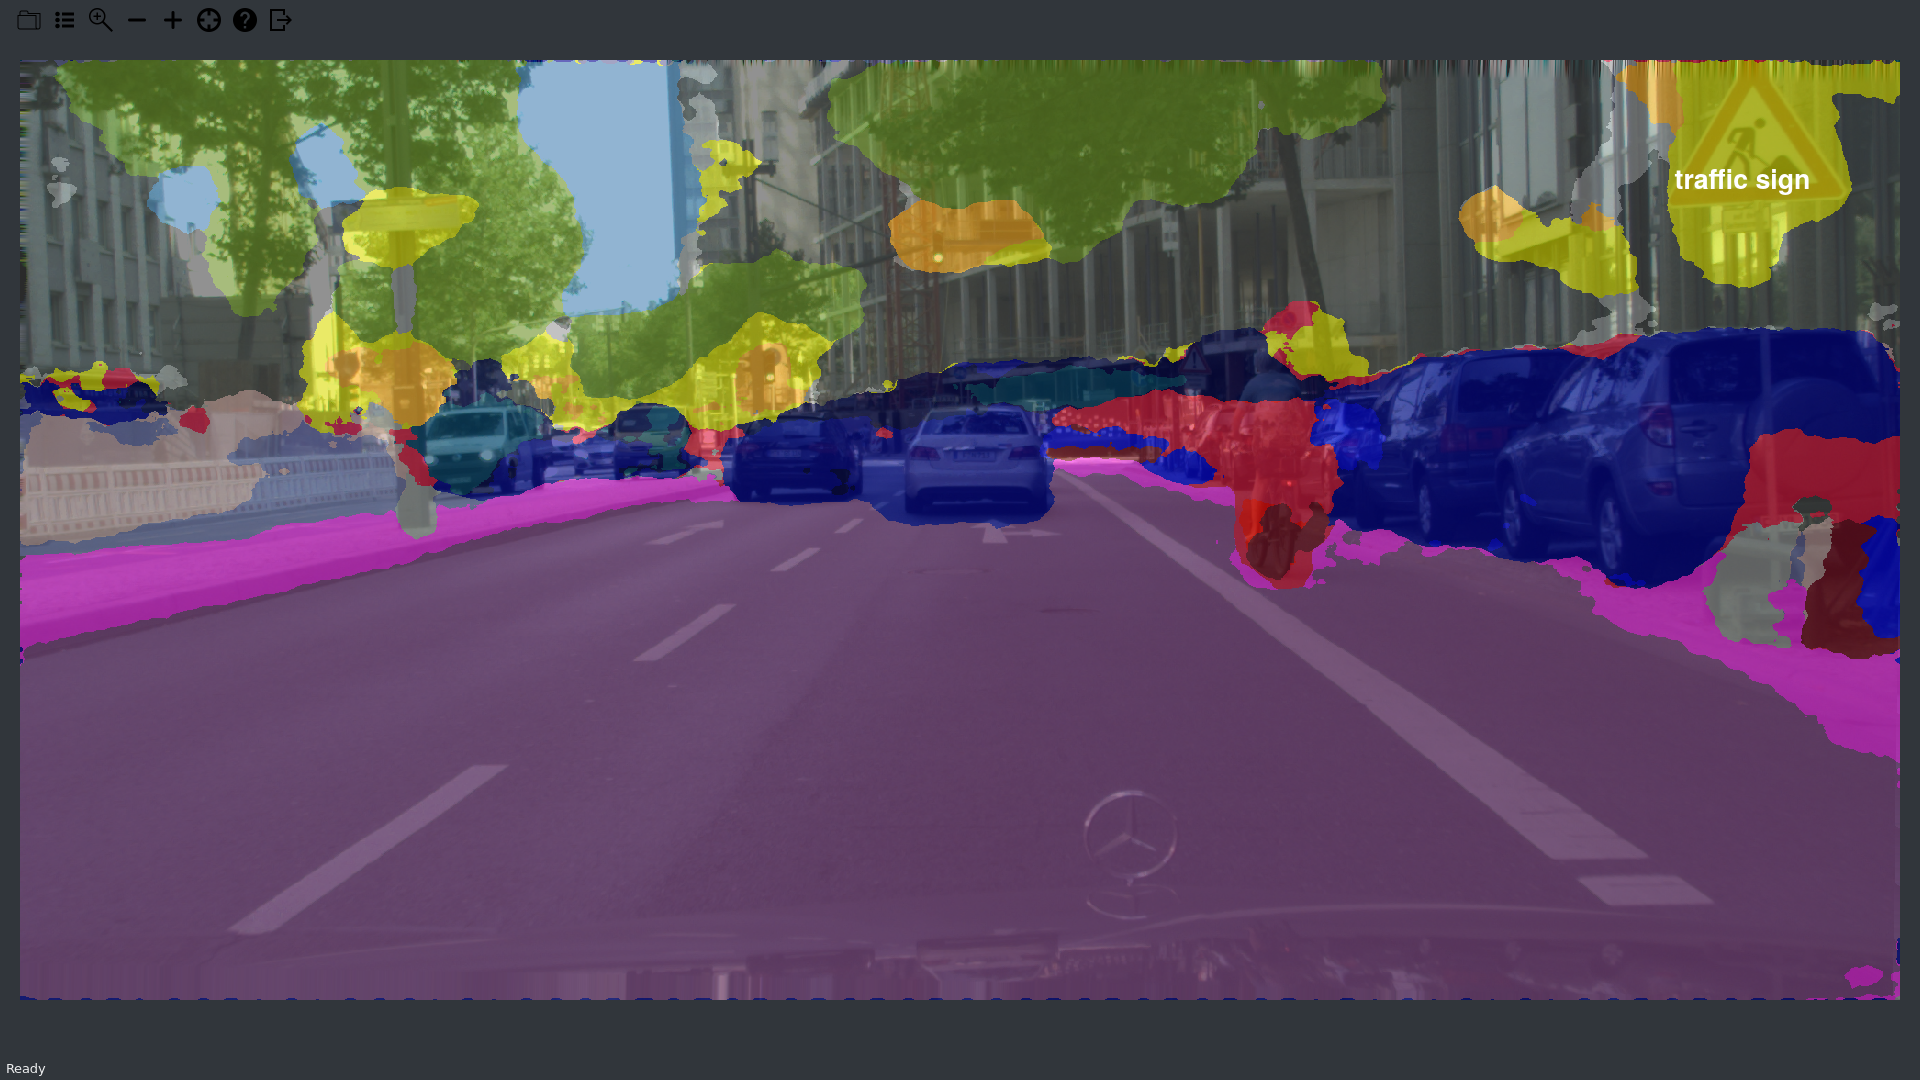
\includegraphics[width=\textwidth, scale=0.3]{Images/viewer_4}
\caption[\textgreek{Παράδειγμα Διαφάνειας}]{\textgreek{Παράδειγμα απεικόνισης ετικέτας σε επιλεγμένο βαθμό διαφάνειας.}}
 \label{fig:viewer_4}
\end{figure}

\textgreek{Τέλος, υπάρχει η δυνατότητα της μεγέθυνσης συγκεκριμένης επιφάνειας της εικόνας στατικού μεγέθους ανάλογα με την θέση που βρίσκεται ο δείκτης από το ποντίκι, δείχνοντας την ετικέτα του κεντρικού εικονοστοιχείου (εικόνα }\ref{fig:viewer_5}).

\begin{figure}[H]
 \centering
 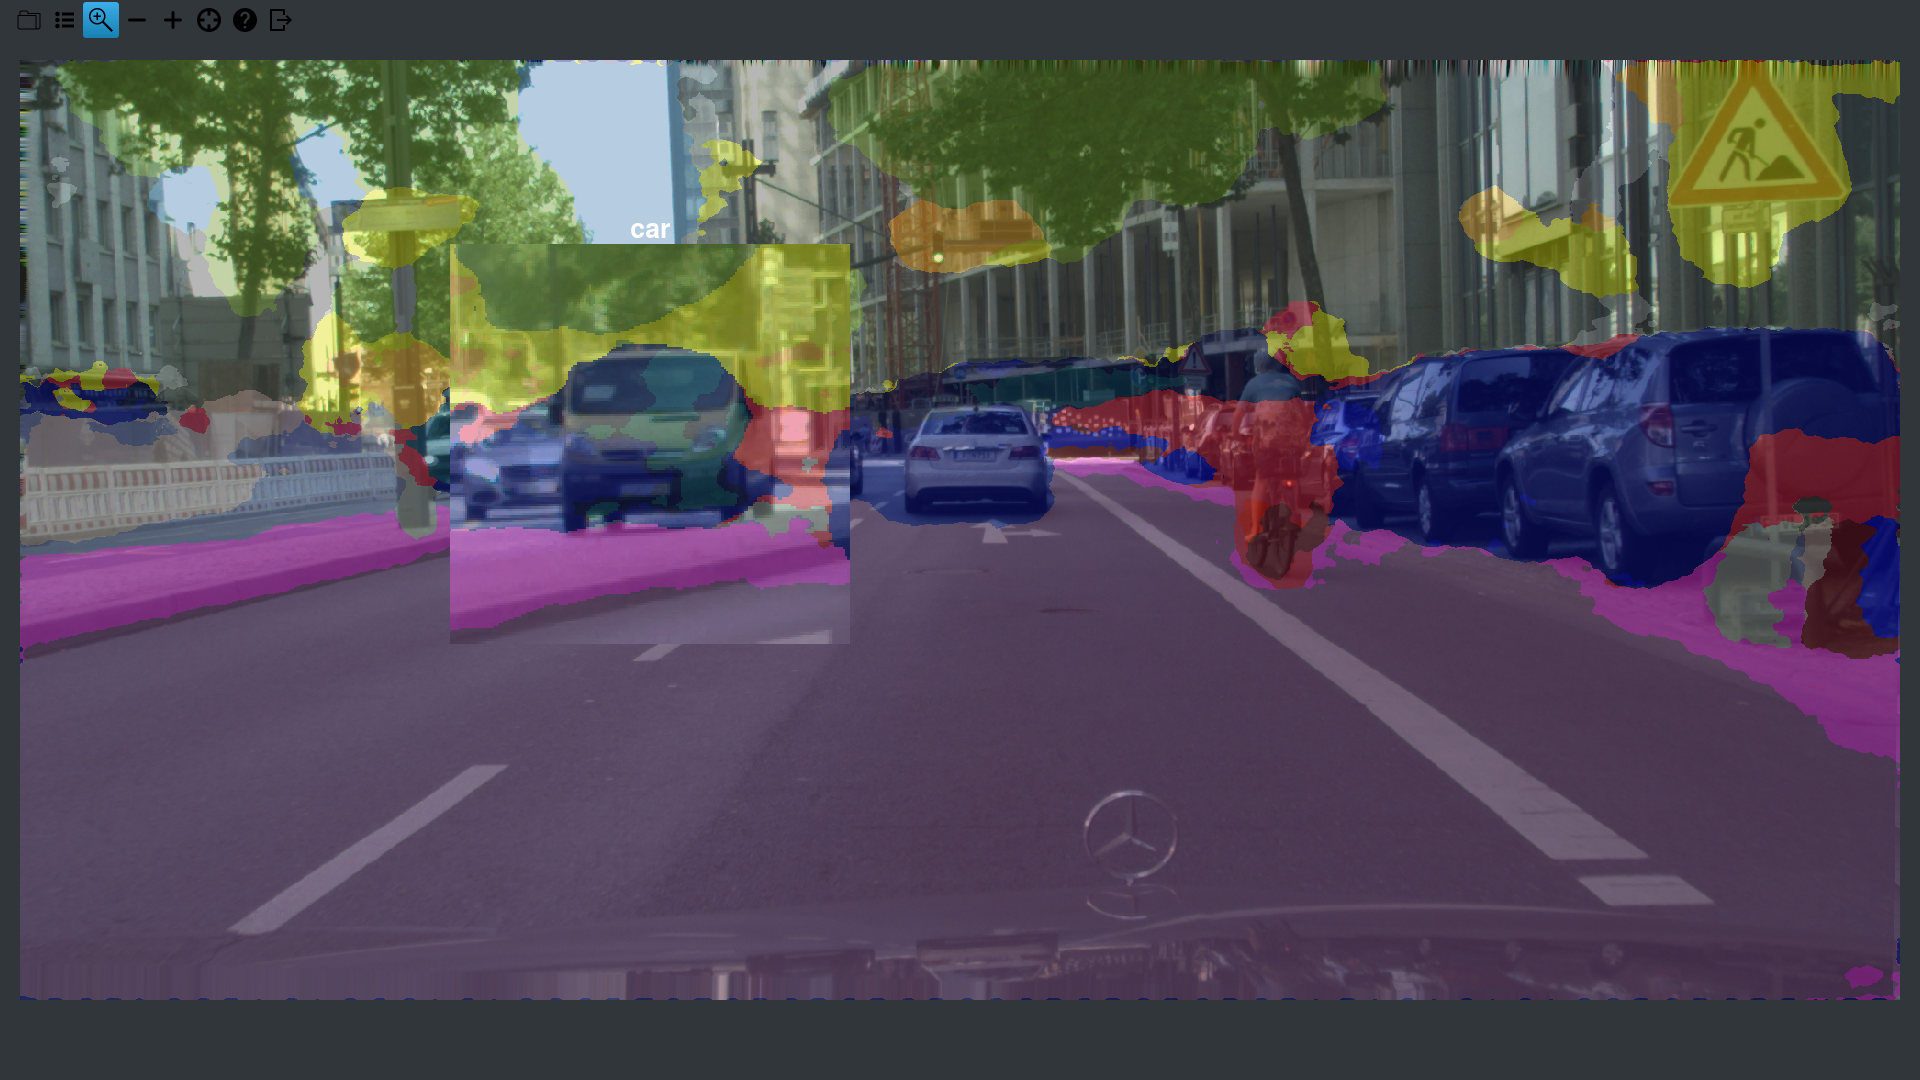
\includegraphics[width=\textwidth, scale=0.3]{Images/viewer_5}
\caption[\textgreek{Παράδειγμα της Λειτουργίας Μεγέθυνσης}]{\textgreek{Λειτουργία μεγέθυνσης επιφάνειας.}}
 \label{fig:viewer_5}
\end{figure}

